\documentclass[12pt, letterpaper]{article}
\usepackage[letterpaper, margin=1in]{geometry}
\usepackage{pdfpages}
\usepackage{listings}
\usepackage{color}
\usepackage{graphicx}
\graphicspath{ {./charts/} }
\setlength{\parskip}{\baselineskip}
\setlength{\parindent}{0pt}
\def\code#1{\texttt{#1}}
\definecolor{dkgreen}{rgb}{0,0.6,0}
\definecolor{gray}{rgb}{0.5,0.5,0.5}
\definecolor{mauve}{rgb}{0.58,0,0.82}

\lstset{frame=tb,
	language=Java,
	aboveskip=3mm,
	belowskip=3mm,
	showstringspaces=false,
	columns=flexible,
	basicstyle={\small\ttfamily},
	numbers=left,
	numberstyle=\tiny\color{gray},
	keywordstyle=\color{blue},
	commentstyle=\color{dkgreen},
	stringstyle=\color{mauve},
	breaklines=true,
	breakatwhitespace=true,
	tabsize=3
}

\begin{document}
\includepdf{cover_page}
\setcounter{page}{1}
\section*{Abstract}

Distributed networks can be developed using various methodologies. 
This article aims to compare various client-server models, including: 
Iterative and Managed/Unmanaged concurrent servers, to track and monitor performance based on time taken to efficiently serve a client. 
The iterative model is generally accepted to be efficient for light request loads whereas concurrent models perform better under heavy request loads. 
The objective of our research is to validate these claims by monitoring heavy and light load requests across the various client/server paradigms and provide the data for analysis.

\section{Introduction}

Our team developed three models to monitor and analyze the performance of client request server calls. 
Each of these models were tested independently using the same metrics to accurately monitor performance. 
According to an article by Daniel A. Menasce, 
``To analyze the performance of client/server systems we need to consider three issues: the anatomy of C/S interactions, the software architecture of a server, and the system architecture which includes hardware configuration and networking topologies'' \cite{menasce}.
The goal of our research was to consider the three issues listed above as they pertain to each protocol tested. 

The first model, Iterative, handles both the connection request and the call. 
The iterative model is implemented through the runnable interface and handles requests one at a time. 
This implementation is appropriate for transactions that are simple and do not require long return times; however, performance suffers when transaction times grow. 
This deficiency in performance is attributed to excessive queuing times resulting from multiple requests. 

The second protocol tested was the concurrent model. 
This model functions similarly to the iterative model; a request is made from the client and the server responds. 
The key differentiator being the concurrent server is capable of spawning child processes, known as a \textit{Thread}, which allows it to handle more than one task at a time. 
Concurrent server performance under a heavy load is much better than the iterative model as there is no queuing delay. 
However, under a light load, the iterative server outperforms the concurrent server which is attributed to the lack of overhead required to spawn a child thread to handle a task. 

The third protocol was implemented using thread pools. 
Thread pools restrict the amount of overhead down to the initialization of the pool. 
In other words, when the threads are created in the pool, they do not close once a task is complete. 
If a thread has finished performing a task, it becomes available for the next request. 
Thread pools typically result in better performance and stability. 
The results of our research indicate that utilizing the thread pool methodology yields the best results overall when tracking performance compared to overhead.
The goal of any network is to provide a timely response to a request. 
When designing a network, it is imperative the engineer understands exactly what is required to complete the task in a manner that does not compromise speed or stability. 
One may assume that a concurrent server is the best option over an iterative server, but as our research indicates, this is not always the case. 
A delicate balance between design and demand must be met to result in optimal performance.
\section{Distributed Application Development}

For this project, we used three different approaches for developing the distributed application: iterative, unmanaged concurrent, and managed concurrent. 
The basic objectives of the project were simple: the server waits for a client to request connection and establishes the connection (Figure 1, line 5), then serves the client in some manner (Figure 1, line 6). 
For this project, serving a client included the client requesting the output from some system command (line 19, 21), the server executing this command (line 23), and returning the results back to the client (line 24).

While each development approach performed the same tasks, the manner in which each did varied slightly. 
Once the server had established a connection with the client, how that client was served was the key differentiator.
The differences, while subtle and small, were found to have large impacts on performance, scalability, and even reliability of the systems involved.

Figure 1:
\begin{lstlisting}
@Override
public void run() {
	while (true) {
		try {
			final Socket client = getNextClient();
			serveClient(client);
		} catch (IOException e) {
			e.printStackTrace();
		}
	}
}

public Socket getNextClient() throws IOException {
	final Socket client = server.accept();
	return client;
}

public void serveClient(Socket client) throws IOException {
	final BufferedReader in = new BufferedReader(new InputStreamReader(client.getInputStream()));
	final PrintStream out = new PrintStream(client.getOutputStream());
	final String read = in.readLine();
	final MenuOption selection = MenuOption.valueOf(read);
	final String response = executeCommand(selection);
	out.println(response);
	out.close();
}
\end{lstlisting}

\subsection{Iterative}

The Iterative server approach is the the simplest of the three. 
It is referred to as ``iterative'' because each client is served iteratively, one at a time, in order. 
The server operates with a single \code{Thread}. 
This Thread is responsible for waiting for a client connection request, establishing the connection once requested, and serving the client. 
Waiting for a client is done using the \code{accept()} method (Figure 1, line 14) found in the \code{SocketServer} class.
This method is known as a \textit{blocking call} because the caller cannot continue until this method finishes. 
That is, \code{accept()} will wait until a client requests connection before continuing.
Once a client connection is established, the same Thread will then serve that client. 
Because the same Thread handles both the connection and the processing, the next client cannot be served until the previous request has completed. Clients will need to \textit{queue}.

\subsection{Concurrent (Unmanaged)}

Concurrent servers are an improvement over Iterative due to a simple, key difference: the client is served on a different Thread than the one that handles the connection requests. 
That is, multiple clients can be served \textit{at the same time}.
The main Thread is still responsible for handling and establishing incoming connection requests, but once a client has connected, a new Thread is created to serve this client (Figure 2, line 3-9). 
This new Thread will run \textit{concurrently}, at the same time, allowing the main Thread to immediately go back to waiting for the next client. 
Clients will not need to queue; as such, there is no \textit{queuing delay}.

Figure 2:
\begin{lstlisting}
@Override
public void serveClient(Socket client) throws IOException {
	new Thread(() -> {
		try {
			super.serveClient(client);
		} catch (IOException e) {
			e.printStackTrace();
		}
	}).start();
}
\end{lstlisting}

While this approach may sound like the best solution, it has its drawbacks: namely the overhead associated with creating a new Thread for each request. 
If, for example, two-hundred clients were to simultaneously make a request, then two-hundred Threads would need to be created. 
This places a lot of strain on the system as the operating system must perform many complex scheduling algorithms for these Threads, which may deprive other applications of the necessary resources to run other, more critical services. 
This is known as \textit{oversubscription} \cite{microsoft}.

\subsection{Thread Pool (Managed Concurrent)}

Managed Concurrent servers can be implemented in several ways, but the objective is the same: limit the number of Threads created to prevent oversubscription. 
In this example, Thread management was achieved using a fixed \textit{Thread Pool}.
A Thread Pool, as the name implies, is a pool of Threads. 
A fixed pool is instantiated with a fixed number of Threads that does not change for the life of the pool.
When you submit a \textit{job} to the pool (Figure 3, line 3-9), a Thread from the pool is removed, used to execute the job, then returned to the pool when the job is complete. 
Each Thread is recycled, removing the need to create a new Thread per-request.
If there are no available Threads in the pool, then the job is queued. 
While this does reintroduce queuing delay as a possibility, it prevents oversubscription, which dramatically improves the stability of the system.

Figure 3:
\begin{lstlisting}
@Override
public void serveClient(Socket client) throws IOException {
	pool.submit(() -> {
		try {
			super.serveClient(client);
		} catch (IOException e) {
			e.printStackTrace();
		}
	});
}
\end{lstlisting} 
\section{Results and Comparison}

\subsection{Test Bed}

Testing was performed on client and server computers with similar specifications. 
Both computers were Dell Optiplex 755 platforms, running the Ubuntu 14.04.4 GNU/Linux operating system. 
The Dells were equipped with Intel Core2 Quad CPU Q9300 processors at 2.50GHz clock speed, with 4 gigabytes of RAM. 
For storage, both machines were equipped with SATA Seagate Barracuda 7200.10 hard drives with a capacity of 160GB, running at 7200 RPM with an 8MB cache at a speed of 3.0Gb/s.

Networking was implemented on the University of North Florida’s VPN, cloudlab.unf.edu, using a Netgear gigabit switch, and both client and server machines were equipped with an Intel 82566DM-2 Gigabit Network Connection. 
The IP address of the client was 192.168.100.111 while the server’s IP was 192.168.100.112.

\subsection{Studies Carried Out}

In order to test the protocols, it is common to use a multistep process 
\cite{stackify}.
Step one is to identify the testing environment. 
All testing was done on the hardware and software provided by the University of North Florida, as specified in section 3.1. 
Second we identify KPIs and performance metrics. 
Performance testing can be broken down into two basic categories, Functional vs. Non Functional testing. 
We were concerned primarily with Non-Functional testing, which tests the readiness of a system as opposed to task-based testing 
\cite{reqtest}.
Non-Functional testing can further be broken down into categories such as load testing, stress testing and spike testing among others. 
For this project we focused on Scalability Testing, which determines how effectively the system handles increasing workloads. 
For corporations with wired, distributed wide area IP data networks, the most requested QoS metrics for business-critical applications are network latency and especially, application response time
\cite{morreale}.
For this test, the metric that was measured was latency, by measuring response time per transaction.

Next it is important to plan how to capture the required metrics. For this test, the team determined to subtract the system time a response was received by the client from the time that the request was sent. This was implemented in the class \code{MultiClientSim} by using a for-loop to iterate through each active client, declaring a \code{startTime} variable using \code{System.currentTimeMillis()} and subtracting an \code{endTime} variable after the server response also using \code{System.currentTimeMillis()}. 

The first series of tests were run using an iterative protocol, measuring the mean server response time as correlating to the number of clients. Both tests stepped through a progression of clients  using the set  $n = \{1, 5, 10, 20, 30, 40, 50, 60, 70, 75\}$.  
The first test measured response times for a \code{netstat} request (graph attachment 1), while the second test measured response time for a \code{date} query (graph attachment 2). 
In the second series of tests, these tests were repeated but with the server process configured to handle multiple client requests concurrently by spawning a thread per request.

\subsection{Results}

The iterative server performs fairly well with a light load requesting date and time, increasing linearly as clients are added and then roughly plateauing after 40 clients. 
The concurrent server does not fare as well with response time rising sharply for the first 30 clients, after which response time levels out. 
Our results showed that the iterative server ranged from a response time of 20 ms to 35 ms as we reached 75 servers.
The concurrent server performed better at higher client levels, peaking at less than 25 ms. 
During the netstat tests, both iterative and concurrent protocol response times increase exponentially. 
For the iterative protocol the response times increase very sharply, reaching over 1000 ms after the first 30 clients to approximately 7500 ms after 75 clients. 
The concurrent protocol clearly performs better on this test, still being around approximately 800 ms after 30 clients and peaking at less than 5000 ms after 75 clients. 

The testing confirmed that the iterative protocol performs better with lighter loads and fewer clients, but the concurrent protocol outperforms as we increase the load and client count.
We saw severe fluctuation during the date and time tests with both protocols between 30 and 75 clients. 
While many performance tests start with a measure of latency, they also typically include other KPIs such as CPU and memory utilization, page file utilization, disk time and amount of free space
\cite{molyneaux}.
Adding some of these extra KPIs on future testing could help explain testing inconsistencies such as fluctuations and high standard deviations.

\section{Conclusion}

For project 1, our team tested client request response time using iterative servers. 
Project 2 tested the same processes using concurrent servers to compare which method performed best to serve a client. 
Before the actual testing of the client servers, we stated that the iterative performs better under a light request load while the concurrent operates better under a heavy request load. 
The printed graphs for the iterative and concurrent tests include both the light and heavy request load. 
Analysis of the light load results suggest the iterative model was faster while under a light request when serving the client. 
The graph for the Iterative model displayed a steadier work progress and showed a decline and decrease after 40 clients. 
The concurrent server under a light load showed there was a decline and decrease after 30 clients. 
This graph shows that iterative performs better when there is a small number of clients as it has the capability to work better and outperforms the concurrent light load. 

After comparing the light load client request, we tested the heavy load and compared the two graphs. 
The iterative server was able to handle the requests very well until there was a decline and decrease in the request after 60 clients, it then picked itself back up and increased the work load past 70 clients. 
The concurrent request was indeed better than the Iterative as it was shown on the graph. The concurrent had a steady increase as more clients were being served but there was no decrease at all during the work for the client. 
the concurrent server was able to demonstrate it could handle heavy requests with little deviation in performance compared to time.

Our team concluded if a request is small, the best method to implement would be an iterative server. 
However, if the request is large, the concurrent server is the better option to ensure optimal performance. 
Our research also shows there is no ``silver bullet'' when building a server. 
One must have many considerations to build a solution that serves requests in a fast and efficient manner.

\pagebreak
\begin{thebibliography}{999}
	
	\bibitem{menasce}
	D. A. Menasce, V. Almeida
	``Performance of Client/Server Systems'',
	in \textit{Performance Evaluation: Origins and Directions},
	Berlin: Springer-Verlag, 2000.
	pp. 201-218.
	
	\bibitem{stackify}
	Stackify.com,
	``The Ultimate Guide to Performance Testing and Software Testing: Testing Types, Performance Testing Steps, Best Practices, and More'', 2017.
	[Online]. Available: https://stackify.com/ultimate-guide-performance-testing-and-software-testing/.
	[Accessed: 18-Nov-2018]
	
	\bibitem{reqtest}
	U. Eriksson,
	``Functional vs Non-Functional Testing'', 2012
	[Online]. Available: https://reqtest.com/testing-blog/functional-vs-non-functional-testing/.
	[Accessed: 18-Nov-18]
	
	\bibitem{morreale}
	E.S.H. Tse-Au and P.A. Morreale,
	``End-to-end QoS measurement: analytic methodology of application response time vs. tunable latency in IP networks'',
	in \textit{Network Operations and Management Symposium Conf.}, 2002 
	
	\bibitem{molyneaux}
	I. Molyneaux, \textit{The Art of Application Performance Testing}.
	Boston: O'Reilly,
	2009
\end{thebibliography}
\pagebreak
\section*{Graphs}
\begin{center}
	Graph 1: Iterative Server Heavy Load\\
	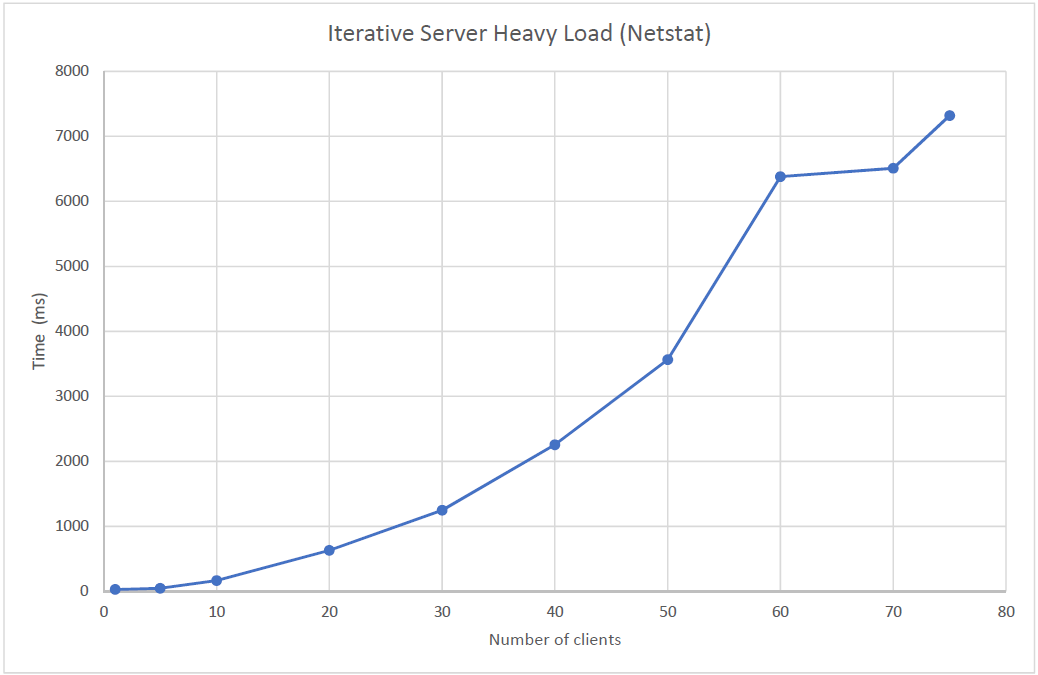
\includegraphics[width=16cm, height=8cm]{iterative-heavy.png}
	
	Graph 2: Iterative Server Light Load\\
	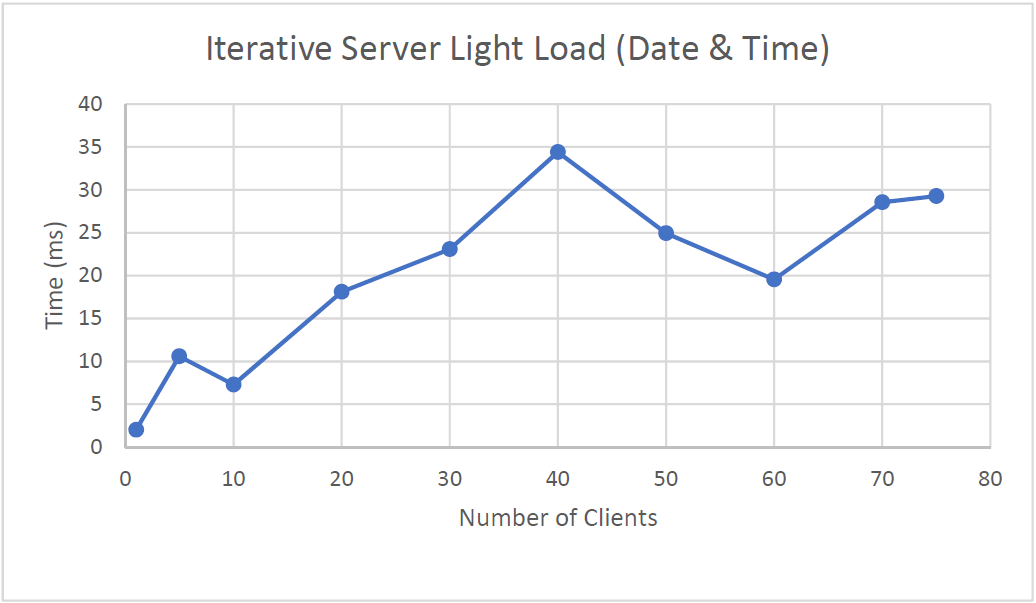
\includegraphics[width=16cm, height=8cm]{iterative-light.png}
	
	\pagebreak
	
	Graph 3: Concurrent Server Heavy Load\\
	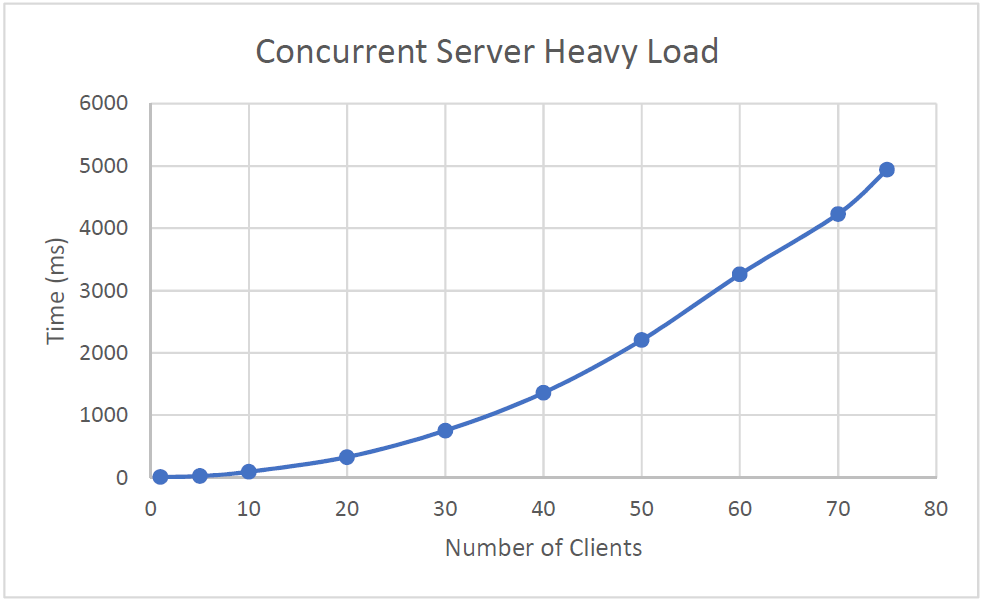
\includegraphics[width=16cm, height=8cm]{concurrent-heavy.png}
	
	Graph 4: Concurrent Server Light Load\\
	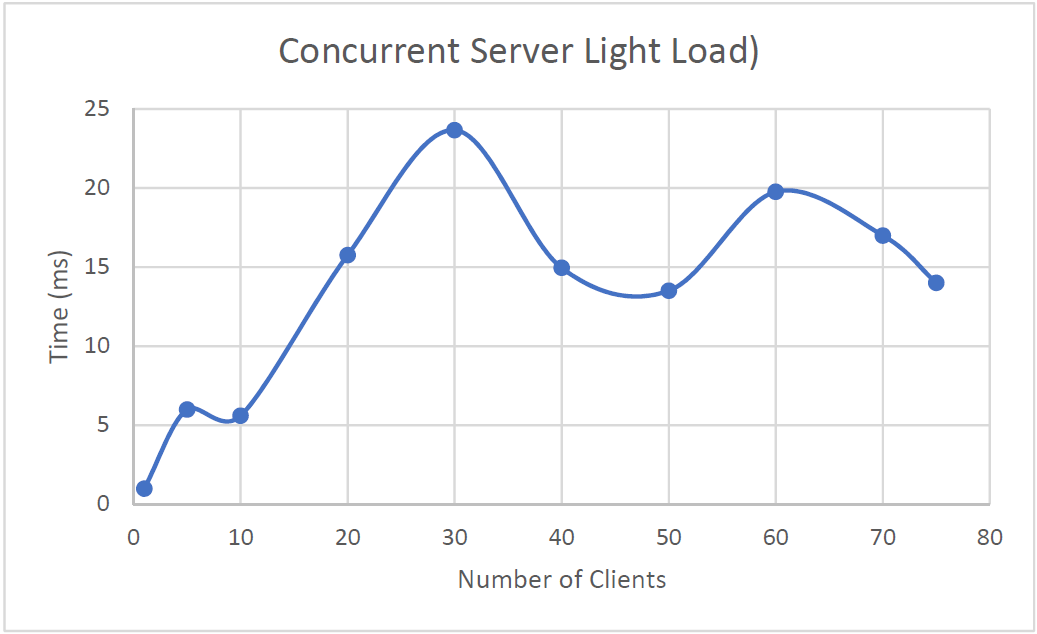
\includegraphics[width=16cm, height=8cm]{concurrent-light.png}
\end{center}

\end{document}